

% File: formatting-instruction.tex
\documentclass[letterpaper]{article}
\usepackage{aaai}



\usepackage{subfig}

\usepackage{tikz}
\usetikzlibrary{shapes}
\usetikzlibrary{positioning}

\usepackage{times}
\usepackage{helvet}
\usepackage{courier}
\usepackage{graphicx}
\graphicspath{{plots/}}

\newcommand{\solver}[1]{{\sc #1}}
\newcommand{\system}[1]{\solver{#1}}
\newcommand{\problem}[1]{{\rm #1}}
\newcommand{\pcogx}{\solver{PCogX}}


\newcommand{\actNam}[1]{\texttt{#1}}
\newcommand{\pp}[1]{\actNam{#1}}

\newcommand{\Expect}{\makebox[1em]{$\mathbin{\mbox{\sf E}}$}}

\newtheorem{definition}{Definition}
\newtheorem{proposition}{Proposition}
\newtheorem{lemma}{Lemma}
\newtheorem{theorem}{Theorem}
\newtheorem{property}{Property}
\newtheorem{corollary}{Corollary}

\newcommand{\laostar}{\textsc{lao$^*$}}
\newcommand{\fastdownward}{\textsc{FastDownward}}


\newcommand{\obsDist}{\ensuremath{\mathit{v}}}

\newcommand{\states}{\ensuremath{\mathcal{S}}}
\newcommand{\state}{\ensuremath{s}}
\newcommand{\observ}{\ensuremath{o}}
\newcommand{\observation}{\ensuremath{\observ}}
%% \newcommand{\percept}{\ensuremath{\widetilde{\observ}}}
\newcommand{\reward}{\ensuremath{{\sf R}}}
\newcommand{\transProb}{\ensuremath{{\sf Pr}}}
%% \newcommand{\States}{\ensuremath{\mathbb{S}}}
%% \newcommand{\TransProb}{\ensuremath{\textbf{Pr}}}
%% \newcommand{\Reward}{\ensuremath{\reward}}
%% \newcommand{\Actions}{\ensuremath{\mathbb{A}}}
%% \newcommand{\Observ}{\ensuremath{\mathbb{O}}}
\newcommand{\observations}{\ensuremath{O}}
\newcommand{\policy}{\ensuremath{\pi}}
\newcommand{\actions}{\ensuremath{\mathcal{A}}}
\newcommand{\action}{\ensuremath{a}}

%% \newcommand{\object}{\ensuremath{o}}
%% \newcommand{\objects}{\ensuremath{\mathcal{O}}}

\newcommand{\bstate}{\ensuremath{b}}

\newcommand{\Omit}[1]{}

\newcommand{\props}{\ensuremath{{\cal P}}}
\newcommand{\prop}{\ensuremath{p}}
\newcommand{\propositions}{\props}
\newcommand{\percepts}{\ensuremath{\Pi}}
\newcommand{\percept}{\ensuremath{\pi}}

\newcommand{\stochActions}{\ensuremath{\actions}}
\newcommand{\detActions}{\ensuremath{\actions^d}}
\newcommand{\stochAction}{\ensuremath{\action}}
\newcommand{\detAction}{\ensuremath{\action^d}}
\newcommand{\stochAct}{\stochAction}
\newcommand{\detAct}{\detAction}

\newcommand{\stochSenses}{\ensuremath{K}}
\newcommand{\detSenses}{\ensuremath{K^d}}
\newcommand{\stochSense}{\ensuremath{\kappa}}
\newcommand{\detSense}{\ensuremath{\kappa^d}}


\newcommand{\poss}{\ensuremath{\pp{poss}}}
\newcommand{\add}{\ensuremath{\pp{ add}}}
\newcommand{\delete}{\ensuremath{\pp{delete}}}



\newcommand{\nodes}{\ensuremath{\mathcal{N}}}
\newcommand{\selections}{\ensuremath{\Psi}}
\newcommand{\transitions}{\ensuremath{\Eta}}
\newcommand{\node}{\ensuremath{n}}
\newcommand{\selection}{\ensuremath{\psi}}
\newcommand{\transition}{\ensuremath{\eta}}


\def\oom{$^{\tt +}$}
\def\zom{$^*$}
\def\bump{\hspace{1cm}}
\newenvironment{tabtt}{\begin{tt}\begin{tabbing}}{\end{tabbing}\end{tt}}%

\nocopyright

\pdfinfo{
/Title (Switching in Continual Planning for Practical Robot Control)
/Subject (Proceedings of the 21st International Conference on Automated Planning and Scheduling)
/Author (NA)}
% The file aaai.sty is the style file for AAAI Press 
% proceedings, working notes, and technical reports.
%
%% \title{Interleaved Serial and Decision-Theoretic Planning for a Mobile Robot}

%% \title{Interleaved Serial and Decision-Theoretic Planning for
%% Practical Robot Control}

% \title{Interleaved Serial and Decision-Theoretic Planning for High-Level Robot Control}

\title{A Switching Planner for Combined Task and Observation Planning}
\author{anonymous}
\setcounter{secnumdepth}{0}


\begin{document} 
\maketitle

\begin{abstract}

%% Those processes must 

From an automated planning perspective the problem of practical mobile
robot control in realistic environments poses many important and
contrary challenges.  On the one hand, the planning process must be
lightweight, robust, and timely. Over the lifetime of the robot it
must always respond quickly with new plans that accommodate exogenous
events, changing objectives, and the underlying unpredictability of
the environment.  On the other hand, in order to exhibit efficient
behaviours the planning process must perform computationally expensive
reasoning about contingencies and possible revisions of subjective
beliefs according to quantitatively modelled uncertainty in acting and
sensing.
%%
Towards addressing these challenges, we develop a \emph{continual
planning} approach that {\em switches} between using a fast
satisficing ``classical'' planner, to decide on the overall strategy,
and decision-theoretic planning to solve small subproblems where
deeper consideration of the sensing model is both practical, and can
significantly impact overall performance. We evaluate our approach
in large problems from a realistic robot exploration domain.

%% partial observability



%% In cooperation with execution monitoring, it must perform repair
%% and/or replanning in order to seamlessly accommodate exogenous events,
%% changing objectives, and the underlying unpredictability of the
%% environment.

%% Realistic robot planning problems in uncertain environments often
%% require achieving tasks while also finding out about the
%% world. Because the world state cannot be observed directly, these
%% problems are naturally represented as partially observable Markov
%% decision problems (POMDPs). However, these are typically intractable
%% for realistic problems.
%%

\end{abstract}

%% \section{Moritz's Initial Outline}

%% \subsection{Switching Planner Outline}

%% Outline the high level approach here:
%% \begin{itemize}
%% \item Problem input (factored initial state, DTPDDL observations)
%% \item Determinisation
%% \item Problem generation for DT
%% \item Belief revision
%% \end{itemize}

%% \subsection{Determinisation}

%% \begin{itemize}
%% \item Generation of deterministic sensing models
%% \item Determinisation of the initial state
%% \item Compiling reward model into (soft-)goal model
%% \item Cost function in FD (maybe this could mentioned in the outline?)
%% \end{itemize}

%% \subsection{Subtask Generation}
%% \begin{itemize}
%% \item Goal generation from CP trace
%% \item Disconfirm actions
%% \item State pruning according to CP trace
%% \end{itemize}

%% \subsection{Belief revision}
%% Not sure if this needs its own section
%% \begin{itemize}
%% \item Convert inital state into bayesian network
%% \item Belief updates with observation nodes
%% \item Create new network for next planning runs
%% \end{itemize}

\section{Introduction}



%% LONG PLANNING HORIZON. MORITZ, CAN YOU PLEASE GIVE ME THE NUMBER OF
%% STEPS IN THE BIGGER PLANS. 

A number of recent integrated robotic systems incorporate a
high-level {\em continual planning} and execution monitoring
subsystem~\cite{wyattetal2010tamd,talamadupula:2010,Kraft2008}.
%%
For the purpose of planning, sensing is modelled
deterministically, and beliefs about the underlying state are
modelled qualitatively.
%%
Both~\citeauthor{talamadupula:2010} and~\citeauthor{wyattetal2010tamd}
identify
continual planning with probabilistic
models of noisy sensing and state as an important challenge for future
research.
%%
Motivating that sentiment, planning according to accurate
stochastic models should yield more efficient and robust
deliberations.
%%
%% In the first place, that means moving from deterministic to
%% probabilistic models of noisy sensing, and from qualitative to
%% quantitative models of state uncertainty. 
%%
In essence, the challenge is to develop a planner that
exhibits speed and scalability similar to planners employed in
existing robotic systems---e.g.,~\citeauthor{wyattetal2010tamd} use a
satisficing {\em classical} procedure---and which is also able to
synthesise relatively efficient deliberations according to detailed
probabilistic models of the environment.


This paper describes a {\em switching} domain independent planning
approach we have developed to address this challenge. 
%%
Our Planner is {\em continual} in the usual sense that plans are
adapted and rebuilt online in reaction to changes to the model of the
underlying problem and/or domain---e.g., when goals are
modified, or when the topological map is altered by a door being
closed.
%%
It is integrated on a mobile robot platform that continuously
deliberates in a stochastic dynamic environment in order to achieve
goals set by the user, and acquire knowledge about its surroundings.
%%
Our planner takes problem and domain descriptions expressed in a novel
extension of PPDDL~\cite{younes:etal:2005}, called {\em
Decision-Theoretic DTPDDL}, for modelling stochastic decision
problems that feature partial observability.  In this paper we
restrict our attention to problem models that correspond to
deterministic-action multi-goal-oriented POMDPs 
% \footnote{We note that
% POMDPs with stochastic actions can be compiled into equivalent
% deterministic-action POMDPs, where all the original action uncertainty
% is expressed in the starting-state
% distribution~\cite{ng:Jordan:2000}.}
in which all actions have
non-zero cost---i.e., an optimal policy can be formatted as a finite
horizon contingent plan. Moreover, we target problems of a size and
complexity that is challenging to state-of-the-art sequential
satisficing planners, and which are too large to be solved directly by
decision-theoretic (DT) systems.

Our planner {\em switches}, in the sense that the base planning
procedure changes depending on our robot's subjective degrees of
belief, and on progress in plan execution. When the underlying planner is
a fast (satisficing) {\em classical} planner, we say planning is in a
{\em sequential} session, and otherwise it is in a DT session.
%%
A {\em sequential} session plans, and then pursues a high-level
strategy---e.g., go to the kitchen bench, and then observe the
cornflakes on it.
%%
A DT session proceeds in a practically sized {\em abstract} process,
determined according to the current sequential strategy and underlying
belief-state.
%%


We evaluate our approach in simulation on problems posed by object search and room categorisation tasks that our indoor
robot undertakes. Those feature a deterministic task planning aspect
with an active sensing problem. The larger of these problems features
$6$ rooms, $25$ topological places, and $21$ active sensing
actions. The corresponding decision process has a number of states
exceeding $10^{36}$, and high-quality plans require very long planning
horizons.
%%
Although our approach is not optimal, particularly as it relies on the
results of satisficing sequential planning directly, we find that it
does nevertheless perform better than a purely sequential replanning
baseline. Moreover, it is fast enough to be used for real-time
decision making on a mobile robot.


%% \section{Propositional Decision-Theoretic Planning}
%% 
We describe the partially observable propositional probabilistic
planning problem, with costs and rewards. We model a process state
$\state$ as the set of propositions that are true of the
state. Notationally, $\props$ is the set of propositions, $\prop$ is
an element from that set, and we have $\state \subseteq
\props$. The underlying process
dynamics are modelled in terms of a finite set of {\em probabilistic
STRIPS operators}~\cite{boutilier:abstraction} $\stochActions$ over
state-characterising propositions $\propositions$.
%%
We say an action $\stochAction \in \stochActions$ is
applicable if its precondition $\poss(\stochAction)$, a set of
propositions, are satisfied in the current state -- i.e., $\poss(\stochAction) \subseteq
\state$. We denote by $\mu_{\stochAction}(\detAction_i)$ the probability that
nature chooses a deterministic STRIPS effect $\detAct_i$, and for
all \stochAction\ we require
$\sum_{\detAction_i \in \detActions(\stochAction)}
\mu_{\stochAction}(\detAction_i) = 1$.

We are concerned with problems that feature partial
observability. Although we could invoke {\em extended probabilistic
STRIPS operators}~\cite{rintanen:01} to model actions and observations
propositionally, we find it convenient for presentation and computation to
separate sensing and action. Therefore, we suppose a POMDP has a
perceptual model given in terms of a finite set of stochastic {\em
senses} $\stochSenses$, deterministic sensing outcomes $\detSenses$,
and perceptual propositions $\percepts$, called {\em percepts}. In
detail, we take an observation $\observ$ to be a set of percepts
$\observ \subseteq \percepts$, and denote by \observations\ the set of
reachable observations. The underlying state of the process cannot be
observed directly, rather, senses $\stochSense \in \stochSenses$
effect an observation $\observ \in
\observations$ that informs what should be believed about the state the
process is in. If $\action$ is applied effecting a
transition to a successor state $\state'$, then an observation occurs
according to the active senses $\stochSenses(\stochAction, \state')
\subseteq \stochSenses$. A sense $\stochSense$ is active, written
$\stochSense \in \stochSenses(\stochAction, \state')$, if the senses'
action-precondition, $\poss_\stochActions(\stochSense)$, is equal to
$\stochAction$, and the state-precondition $\poss_\states(\stochSense)
\subseteq \propositions$ is satisfied by the state $\state'$ -- In the
usual sense that \mbox{$\poss_\states(\stochSense)\subseteq\state'$}.
%%
When a sense is active, nature must choose exactly one outcome amongst
a small set of deterministic choices $\detSenses(\stochSense)
\equiv \{\detSense_1, \ldots, \detSense_k \}$, so that for each
$i$ we have $\detSense_i \subseteq \percepts$. The probability of
the $i^{th}$ element being chosen is given by
$\psi_{\stochSense}(\detSense_i)$, where $\sum_{\detSense_i \in
\detSenses(\stochSense)} \psi_{\stochSense}(\detSense_i) =
1$. The observation received by the agent corresponds to the union of
perceptual propositions from the chosen elements of active
senses.

A POMDP has a starting configuration that corresponds to a Bayesian
belief-state. Intuitively, this is the robot's subjective belief about
its environment. Formally, a belief-state $\bstate$ is a probability
distribution over process states. We write $\bstate(\state)$ to denote
the probability that the process is in $\state$ according to
$\bstate$, and $\bstate_0$ when discussing the starting
configuration. 

%% Finally, we make some fairly standard assumptions. First, that action
%% execution and sensing occur instantaneously, and that only one action
%% can be applied per plan-step. Secondly, it can arise that in some
%% states an action is applicable, and in others it is not. Moreover, a
%% belief-state can assign non-zero probability to states where that
%% applicability holds, and states where it does not. %% We differ
%% %% from~\citeauthor{younes:littman:04}~(\citeyear{younes:littman:04})
%% %% In beliefs where an action exists that is applicable in some state 
%% %% with non-zero probability, and not applicable in another, we differ
%% %% from~\citeauthor{younes:littman:04}~(\citeyear{younes:littman:04}),
%% %% because 
%% %% in that
%% %% we forbid the execution of the action.
%% %% actions that are not applicable in
%% %% any state of the current belief.  
%% %% Also,
%% Unlike~\citeauthor{hoffmann:brafman:2006}~(\citeyear{hoffmann:brafman:2006}),
%% we incorporate a PPDDL-like default semantics, treating an action
%% \stochAction\ executed at $\state_i$ as if it has no effect at
%% states $\state$ if $\poss(\stochAction) \not\subseteq
%% \state$.

% Mucked around with this, then realised the two sentences were
% contradictory. If we forbid actions applicable in one state but not
% another in the belief state, then clearly we aren't using a
% PPDDL-like semantics.
%% Doubled comments are stuff I added, then removed.

\subsection{Costs, Rewards, and Belief Revision}

Until now we have discussed the POMDP in terms of propositions and
percepts. In order to address belief revision and utility it is
convenient to consider the underlying decision process in a flat
format. This is given by the tuple
$\langle \states, \bstate_0, \actions, \transProb, \reward,
\observations, \obsDist \rangle$. Here, $\bstate_0$ is the initial
belief-state, \states\ is the finite set of reachable propositional
states, \actions\ is the finite set of actions, and \observations\ is
the finite set of reachable observations (i.e., perceptual states).
Where $\state, \state' \in \states$, $a \in \actions$, from $\mu$ we
have a state transition function $\transProb(\state, \action,
\state')$ giving the probability of a transition from state $s$ to
$s'$ if $a$ is applied. For any $\state$ and $\action$ we have
$\sum_{\state' \in \states} \transProb(\state, \action, \state') = 1$.
%%
The function $\reward:\states \times \actions \to \Re$ is a bounded real
valued reward function. Therefore a finite positive constant $c$
exists so that for all $\state \in \states$ and $\action \in
\actions$, $|\reward(\state, \action)| < c$. We model costs as
negative rewards.
%%
From $\psi$ we have that for each $\state' \in \states$ and action
$\action \in \actions$, an observation $\observ \in \observations$ is
generated independently according to a probability distribution
$\obsDist(\state', \action)$. We denote by $\obsDist_\observ(\state',
\action)$ the probability of getting observation $\observ$ in state
$\state'$. For $\state'$ and $\action$ we have $\sum_{\observ \in
\observations} \obsDist_\observ(\state', \action) = 1$.

Successive state estimation is by application of Bayes'
rule.  Taking the current belief $\bstate$ as the {\em prior}, and
supposing action $\action$ is executed with perceptive outcome
$\observ$, the probability that we are in $\state'$ in the
successive belief-state $\bstate'$ is:

\begin{equation}\label{eq:revision}
\bstate'(\state') = \frac{\obsDist_\observ(\state', \action)
  \sum_{\state\in \states} \transProb(\state, \action, \state') \bstate(\state) }{\pp{Pr}(\observ | \action, \bstate)}
\end{equation}

\noindent where $\pp{Pr}(\observ | \action, \bstate)$ is the
normalising factor, that is, the probability of getting observation
$\observ$ given we execute $\action$ in $\bstate$.

\subsection{Plan Evaluation}

An optimal solution to a finite-horizon POMDP is a contingent plan,
and can be expressed as a mapping from observation histories to
actions. Although suboptimal in general, useful plans can also take a
classical sequential format. This is the case in {\em conformant}
planning, where the objective is to find a sequence of actions that
achieves a goal ---i.e., reaches a state that satisfies a given
Boolean condition--- with probability $1$.  Generally, whatever the
plan format, its value corresponds to the expected reward:

%% More generally, a useful
%% formalism for representing solutions to POMDPs is the finite-state
%% controller (FSC). This is a three-tuple $\langle \nodes, \selection,
%% \transition \rangle$ where: $\node \in \nodes$ is a set of controller
%% states, $\selection_\node(\action) = P(\action | \node)$ gives the
%% probability that the controller prescribes \action\ when in state
%% \node, and $\transition_\node(\action, \observation, \node') =
%% P(\node'|\node, \action, \observation)$ gives the probability the
%% controller transitions to state $\node'$, supposing we execute
%% \action\ in state \node\ receiving observation \observation. When
%% acting for finite $N$ steps from controller state $n$, the value of a
%% controller corresponds to the expected cumulative reward:

\begin{equation}\label{eq:expectedvalue}
V_{\pp{PLAN}}(\bstate) = \Expect \bigg{[} 
\sum_{t=0}^{N-1}  \reward(\bstate_t, \pp{PLAN}_t) \mid \pp{PLAN}, \bstate_0 = \bstate \bigg{]}
\end{equation}

\noindent Where $b_t$ is the belief-state at step $t$, $\pp{PLAN}_t$ is
the action prescribed at step $t$, and

\[\reward(\bstate, \action) = \sum_{\state \in \states}
\bstate(\state)\reward(\state, \action).\] 

%% \noindent Finally, it is
%% useful to note that there is a corresponding deterministic FSCs for
%% both sequential (e.g., conformant) and contingent plan formats.



\section{Background and Related Work}



%%  and
%% using various techniques to manage the large state
%% space

%% \citeauthor{hippo-jnl}~(\citeyear{hippo-jnl}) take this
%% approach in a 



Addressing task and observation planning specifically, there have been
a number of recent developments where the underlying problem is
modelled as a POMDP.
%%
For vision algorithm
selection,~\citeauthor{hippo-jnl}~(\citeyear{hippo-jnl}) exploit a
natural hierarchical decomposition of the underlying POMDP into
subproblems where decision-theoretic planning is reasonably
fast. \citeauthor{doshi08:pref_elic}~(\citeyear{doshi08:pref_elic})
represent a preference elicitation problem as a POMDP and take
advantage of symmetry in the belief space ---essentially the idea that
it does not matter what the value of the variable you are trying to
observe is--- to exponentially shrink the state space. Although we
have been actively exploring the \citeauthor{doshi08:pref_elic}
approach, those exploitable structures are not present in problems we
have considered so far due to the task planning requirement. 
%%
%%
Finally,
our approach is in a similar vein to the more classical {\em
dual-mode} control~\cite{cassandra96actingunder}, however in our case
entropy reduction is targeted by planning in an abstract process which
is informed by one execution trace ---computed by a {\em classical}
planner--- and the underlying belief-state.


More generally, there has been much recent work on scaling POMDP
solution procedures to medium-sized
instances~\cite{shani:etal:08,KurHsu08}. In that
setting \citeauthor{kurniawati:etal:2010}~(\citeyear{kurniawati:etal:2010})
recently addressed an inefficiency of offline point-based techniques
in problems with medium length planning horizons, however their
approach take tens of minutes to good plans, and only scales to tens
of thousands of states. In the case of general domain-independent
factored systems, the state-of-the-art scales to relatively small
problems with $2^{22}$ states~\cite{shani:etal:2008}. At their limit,
these procedures take over an hour to converge, and $\sim10$ seconds
on average to perform a single Bellman backup.  For classes of POMDP
that feature exploitable structures (e.g., no actions with negative
effects), problems with as many as $10^{30}$ states can be targeted by
such offline procedures~\cite{brunskill:russell:2010}. Moving someway
towards addressing real-time decision making, recent online POMDP
solution procedures have been developed which can exploit highly
approximate value functions -- typically computed using a point-based
procedure -- and heuristics in forward
search~\cite{ross:etal:2008}. Their applicability in our setting is
limited, firstly because they only scale to smaller problems, with
thousands of states, and also due to the large amount of
\emph{problem-specific} offline processing that might be required to get useful
search guidance. A {\em very} recent and promising online approach for
large POMDPs employs Monte-Carlo sampling to break the curse of
dimensionality in situations where goal reachability is {\em easily}
determined~\cite{silver:veness:2010}.


%% Although we suppose it an interesting
%% item for future work to pursue that direction, it should be noted that
%% ease of goal reachability is not guaranteed in the problems we face,
%% and is certainly not a property to be assumed in domain independent
%% planning.


In the direction of leveraging {\em classical} systems/approaches for
planning under uncertainty, the most highlighted system to date has
been \system{FFR$_a$}~\cite{yoon:etal:2007}; The winning entry from
the probabilistic track of the 2004 International Planning
Competition.  In the continual paradigm, \system{FFR$_a$}
uses \system{FF} to compute sequential plans and execution traces.
%%
More computationally expensive approaches in this vein combine
sampling strategies on valuations over {\em runtime variables} with
deterministic planning procedures~\cite{yoon:etal:2008}. %% The outcome is typically a more
%% robust sequential plan, or contingent
%% plan~\cite{majercik:2006}. 

Also leveraging deterministic planners in problems that feature
uncertainty, \system{Conformant-FF}~\cite{hoffmann:brafman:2006} and
$T_0$~\cite{palacios:geffner:2009} demonstrate how conformant planning
---i.e., sequential planning in unobservable worlds--- can be modelled
as a deterministic problem, and therefore solved using sequential
systems. In this conformant setting, advances have been towards
compact representations of beliefs amenable to existing best-first
search planning procedures, and lazy evaluations of beliefs. Most
recently this research thread has been extended to contingent planning
in fully observable non-deterministic
environments~\cite{albore:etal:2009}.
%%
%% The continual planning system that motivated our
%% project~\cite{brenner:nebel:jaamas09} also has this characteristic,
%% and has been applied in completely observable domains, particularly
%% those featuring multiple communicating agents. 

%% The use of knowledge
%% operators in domains allows plans that act to gain knowledge, but the
%% approach assumes that such actions are deterministic and reliable, an
%% assumption that we relax.



%%No! They simply haven't been evaluated in PO settings. They may, or
%%may not struggle. They have sampling of traces, and that would
%%include observations, and therefore evolutions of beliefs. SSAT was
%%proposed by Littman for POMDPs. So the majercik stuff is perfectly
%%suited to POMDPs.

% Normally if we are going to compare with related work, we do
% actually *compare*. Why didn't you try those approaches? I think
% it's safe to say that FFR will struggle. Why would it even include
% in its plan an observational action that doesn't change the world?

%%
%% However, as we said in the introduction,
%% all these approaches struggle in partially observable domains as they
%% rely on being able to determine the state at all times.


\section{Planning Language and Notations}

The modelling language of choice for planning in probabilistic
problems is the Probabilistic Planning Domain Definition
Language~\cite{younes:littman:04,younes:etal:2005}. PPDDL was used in
all 3 of the International Planning Competitions since 2004. A
variation on PDDL for describing domains with stochastic actions and
uncertain starting configurations, PPDDL is a declarative first-order
language that facilitates factored descriptions of domains and problem
instances. There are straightforward compilations from problems
expressed compactly in PPDDL to propositional representations amenable
to state-of-the-art planning procedures.

Because PPDDL cannot model domains that feature partial observability,
we develop an extension of that language, called Decision-Theoretic
(DT)PDDL. This can express probabilistic models of the sensing
consequences of acting, to quantitatively capture unreliability in
perception. That expressive power is achieved by incorporating
perceptual analogues of fluent, predicate, and action definitions. In
detail, we have declarations of state characterising predicate and
fluent symbols according to the PPDDL syntax. In addition, we allow
two other declarations, for perceptual predicates and fluents
respectively. For example, suppose our robot is tasked with exploring
{\em locations} in order to identify the whereabouts of a {\em
visual-object}. We must describe state and perceptual facts that model
the {\em true}, resp. perceived, locations of objects. In DTPDDL,
these declarations appear as:

\small
\begin{tabtt}
(\=:functions  ;; state fluents\\
  \> (is-in ?v - visual-object) - location )\\
(:observable-functions  ;; perceptual fluents\\
  \> (o-is-in ?v - visual-object) - location )
\end{tabtt}
\normalsize

\noindent To model the sensing capabilities of the agent, we have
operator-like declarations, with preconditions expressed using state
predicate and action function symbols, and uniformly positive effects
over perceptual predicates. A sense declaration corresponds to a
lifted description of proposition {\em senses}. Whereas the effects of
an {\em operator} schema describe how states change under application
of actions, the effects of a {\em sense} schema are perceptual,
specifying the composition of an observation following the execution
of an action. 

%% Also, and without a loss of generality, we find it
%% convenient to separate the actional precondition from the state
%% precondition.

Making the above ideas concrete with an example, suppose a robot
called $\pp{DORA}$ is able to look for a visual-object, such as a
$\pp{box}$, at a given place. We can model that deterministic action
using the following operator schema:


\small
\begin{tabtt}
(\=:action look-for-object \+ \\
   :parameters (\=?r - robot ?v - visual-object\\
   \> ?l - location) \\
   :precondition (and (= (is-in ?r) ?l) ) \\
   :effect (and (assign (reward) -3) ) ) \\
\end{tabtt}
\normalsize


\noindent In a slight departure from PPDDL, we suppose that
$\pp{look-for-object}$ has an effect on the state. That is, its
execution incurs an instantaneous penalty, $3$, that corresponds to
the {\em cost} of performing the visual search.\footnote{In PPDDL {\em
reward} is a {\em reserved word}, and occurs in {\em increased} and
{\em decreased} terms in operator schemata. In that setting, {\em
reward} is interpreted as accumulated, whereas in DTPDDL it is
instantaneous.}

Completing the example, we model the sensing outcome that results from
instantiating the $\pp{look-for-object}$ operator:

\small
\begin{tabtt}
(\= :sense vision \+\\
 :parameters \= (\= ?r - robot ?v - visual-object\\
 \>\>  ?l - location) \\
 :execution \> ( \> look-for-object ?r ?v ?l) \\
 :precondition (and (= (is-in ?r) ?l) ) \\
 :effect \>  (  \> and (when (= (is-in ?v) ?l) \\
   \> \> (probabilistic 0.8 \\
   \>  \>(= (o-is-in ?v) ?l))) \\
  \> (when (not (= (is-in ?v) ?l)) \\
   \>  \> (probabilistic 0.1 \\
   \>  \> (= (o-is-in ?v) ?l))))) \\
\end{tabtt}
\normalsize


\noindent Here, the {\em execution} declaration is a lifted description of
the sense action-precondition -- i.e,
$(\pp{look-for-object}~\pp{DORA}~\pp{box}~\pp{office}) =
\poss_\stochActions(\pp{vision}~\pp{DORA}~\pp{box}~\pp{office})$. Above,
we include a redundant state-precondition, $(=(\pp{is-in}~?r)?l)$ in
order to fully demonstrate the syntax. Interpreting the above schema,
if action $(\pp{look-for-object}~\pp{DORA}~\pp{box}~\pp{office})$ is
executed, there is a $0.8$ chance of perceiving the box if it is in
the $\pp{office}$, and otherwise a $0.1$ chance of perceiving it.

The syntax and semantics for describing initial state distributions in
DTPDDL is taken verbatim from PPDDL. It is useful to present that
factored tree-like structure here, in order to aid us when discussing
our switching continual planner. The distribution is expressed in a
tree-like structure of terms. Each term is either: (1) atomic, e.g., a
state proposition such as $(=(\pp{is-in}~\pp{box})~\pp{office})$, (2)
probabilistic, e.g., $(\pp{probabilistic}~\prob_1 (T_1) .. \prob_n
(T_n))$ where $T_i$ are conjunctive, or (3) a conjunct over
probabilistic and atomic terms. The root term is always conjunctive,
and the leaves are atomic. For example, the starting distribution for
$\pp{DORA}$ might be described as follows:\footnote{In PDDL,
$(\pp{:init}~T_1..T_n)$ expresses the conjunctive root of the tree --
i.e., the root node $(\pp{and}~T_1..T_n)$. Also, we shall write
$\prop$, rather than $(\pp{and}~\prop)$, for conjunctive terms
that contain a single atomic subterm.}

\small
\begin{tabtt}
(\=:init (= (is-in DORA) kitchen) \+ \\
       (probabilistic \=.8 (= (is-in box) office)  \\
		      \>.2 (= (is-in box) kitchen)) \\
       (probabilistic .3 (= (is-in cup) office)  \\
		      \>.7 (= (is-in cup) kitchen))) \\
\end{tabtt}
\normalsize


\noindent The interpretation of such an expression can be given
according to a {\em visitation} of terms. An atom is {\em visited} iff
its conjunctive parent is visited, and a conjunctive term is visited
iff all its immediate subterms are visited. A probabilistic term is
visited iff its conjunctive parent is visited, and exactly one of its
subterms, $T_i$, is visited. Each visitation of the root term
according to this recursive definition encapsulates a starting state,
along with the probability that it occurs. The former corresponds to the
union of all visited atoms, and the latter corresponds to the product
of $\prob_i$ entries on the visited subterms of probabilistic
elements. Making these ideas concrete, our example yields the
following flat state distribution:


\small
\begin{tabular}{cccc}
\hline
Probability & (is-in DORA)  & (is-in box)  & (is-in cup) \\
\hline
.24 & kitchen & office & office \\
.06 & kitchen & kitchen & office \\
.56 & kitchen & office & kitchen \\
.14 & kitchen & kitchen & kitchen \\
\hline
\end{tabular}
\normalsize

From hereon, in order to simplify the discussion (and implementation)
we shall restrict our attention to POMDPs with deterministic
actions. It is worthwhile noting that any POMDP with stochastic
actions can be compiled into an equivalent deterministic-action POMDP,
where all the original action uncertainty is expressed in the
starting-state distribution~\cite{ng:Jordan:2000}. In our setting,
that of finite-horizon planning, such a compilation yields a finite
flat representation of the original POMDP, only with deterministic
actions.


\section{Switching Continual Planner}

We now describe our {\em switching} planning system that operates
according to the continual planning paradigm, given a description of
the current problem and domain in DTPDDL. The system {\em
switches}, in the sense that planning proceeds in interleaved
sessions, in which the base planner is either {\em sequential}/linear
or {\em decision-theoretic}.
%%
During a sequential session, a rewarding {\em trace} of a possible
execution is computed using a cost-optimising satisficing planner
which trades action costs, goal rewards, and determinacy.
%%
Formatted as a linear plan, the trace specifies a sequence of actions
that achieves some reachable goals following a deterministic
approximation of the problem at hand.
%%
Structurally, a trace is a sequence of elements that are either: (i) ground
actions from the DTPDDL description of the world, or (ii) atomic {\em
assumptions}, modelled as deterministic actions, made about the truth
value of facts that can only be determined at runtime (e.g., that a
box of cornflakes is located on the corner bench in the kitchen).
%%
The system always begins in a sequential session, so that plan
execution proceeds by applying DTPDDL actions from the trace, in
sequence, until the outcome of executing the next scheduled action is
too uncertain according to a threshold parameter~(here, 95\%). In that
eventuality a DT session commences, which tailors sensory processing
to determine whether the assumptions made in the trace hold, or which
otherwise acts to achieve the goals.


Because online DT planning in large problems is impractical (we seek
response times in seconds), a DT session plans for an abstract process
determined by the current trace and underlying belief-state. That
abstract problem is characterised by a limited number of propositions,
chosen due to their {\em relevance} to the action whose scheduled
execution triggered the switch to the DT session.
%%the subproblem the DT session is asked tosolve.
% MOG: Describe this in detail in the appropriate subsection
%  This
% abstraction is constructed by first excluding all propositions (and
% related actions) that are not true, or {\em assumed } true, of states
% in the trace, then adding them back, using as an heuristic the entropy
% of the trace assumptions conditional on a candidate
% proposition. Propositions are added, one at a time, until the number
% of states in the initial belief-state reaches a given
% threshold.\footnote{Our experiments are performed using a number of
% different threshold parameters.} 
To that abstract model we also add {\em disconfirm} and {\em confirm}
actions that the DT session can schedule in order to judge an atomic
assumption in the trace. Those actions yield a relatively small reward
if the corresponding judgement is true (or small penalty
otherwise). If a judgement action is scheduled for execution the DT
session is terminated, and control is returned to a new sequential
session.

Whatever the session type, our continual planner maintains a factored
representation of successive belief-states by performing belief
revision. As an internal representation of the $(\pp{:init})$
declaration, we keep a tree-shaped Bayesian network which gets updated
whenever an action is performed, or an observation received. That
belief-state representation is used: (1) as the source of candidate
determinisations for sequential planning, (2) in determining when to
switch to a DT session, and (3) as a mechanism to guide construction
of an abstract process for DT sessions.

\subsection{Sequential Sessions}

As we only consider deterministic-action POMDPs, all state
uncertainty is expressed in the $(\pp{:init})$ declaration. This
declaration is used by our approach to define the starting state for
sequential sessions, and the set of state-assumptions available to
sequential planning.  Writing \#\ if the value of a proposition is
unspecified, taking the $(\pp{:init})$ example from the previous
section, we have the following assumptions:

\small
\begin{tabular}{cccc}
\hline
Probability & (is-in R2D2)  & (is-in box)  & (is-in cup) \\
\hline
%% .24 & kitchen & office & office \\
%% .06 & kitchen & kitchen & office \\
%% .56 & kitchen & office & kitchen \\
%% .14 & kitchen & kitchen & kitchen \\
.7 & kitchen & \# &  kitchen\\
.3 & kitchen & \# & office \\
.8 & kitchen & office & \# \\
.2 & kitchen & kitchen & \# \\
1.0 & kitchen & \# & \# \\
\hline
\end{tabular}
\normalsize

\noindent Each assumption corresponds to one distinct {\em
relaxed} visitation of the root term. Here, a conjunctive term is
visited iff its atomic subterms are visited, and zero or one of its
immediate probabilistic subterms are visited. For a sequential
session, the starting state corresponds to an assumption (usually
unique) with probability $1$.\footnote{To simplify the discussion, we
suppose that the root term of $(\pp{:init})$ lists all atoms that are
necessarily true.} In our example, that starting state is:

\vspace{-1ex}

\small
\[
\begin{array}{l}
\state_0 \equiv \{(=(\pp{is-in}~\pp{R2D2})~\pp{kitchen}),\\
\;\;(=(\pp{is-in}~\pp{box})~\#), (=(\pp{is-in}~\pp{cup})~\#)\}.
\end{array}
\]
\normalsize

\vspace{-1ex}

Encapsulating state-assumptions, we annotate the problem posed during
a sequential session with an \emph{assumptive action} $\assumptiveS{i}$ for
each element $\prob_i (T_i)$, of each probabilistic term from
$(\pp{:init})$. Here, $\assumptiveS{i}$ can be executed if no
$\assumptiveS{j}$, $j \neq i$, has been executed from the same
probabilistic term, and, either
$(\pp{probabilistic}~..\prob_i~(T_i)..)$ is in the root conjunct, or
it occurs in $T_k$ for some executed $\assumptiveS{k}$.
%%
We also add constraints that forbid scheduling of
assumptions about facts after actions with preconditions or effects
that mention those facts. For example, the robot cannot assume it is
plugged into a power source immediately after it unplugs itself.
%%
Executing $\assumptiveS{i}$ in a state $\state$ effects a transition
to a successor state $\state^{T_i}$ with probability $\prob_i$, and
$\state^\bot$ with probability $1 - \prob_i$. Here, $\state^{T_i}$ is
the union of $\state$ with atomic terms from $T_i$. State
$\state^\bot$ is an added sink.


We now describe the optimisation criteria used during sequential
sessions. Where $\prob_i$ is the probability that the $i^{th}$
sequenced action, $\action_i$, from a trace of state-action pairs
$\langle \state_0, \action_0,\state_1, \action_1,.., \state_N \rangle$
does not transition to $\state^\bot$, we have that the optimal trace
has value:

\small
\[
V^* = \max_N \max_{\state_0, \action_0,.., \state_N} \prod_{i=1..N-1} \prob_i \sum_{i=1..N-1}
\reward(\state_i, \action_i),
\]
\normalsize

\noindent  Here,  $\reward(\state_i, \action_i)$ is the instantaneous
reward ---i.e., can be negative for action costs, or positive for goal
achievement--- received for executing action $\action_i$ in state
$\state_i$. Finally, it is worth clarifying that in practise we do not
artificially limit the length of traces that the sequential planner
can consider. Moreover, for problems we consider there is always a
finite optimal trace.

\subsection{DT Sessions}

When an action is scheduled whose outcome is uncertain according to
the underlying belief-state, the planner switches to a DT
session. That plans for {\em small} abstract processes defined
according to the action that triggered the DT session, the assumptive
actions in the proceeding trace, and the current
belief-state. Targeted sensing is encouraged by augmenting the reward
model to reflect a heuristic value of knowing the truth about
assumptions. In detail, all rewards from the underlying problem are
retained. Additionally, for each relevant assumptive action
$\assumptiveS{i}$ in the current trace, we have a {\em disconfirm
action} $\assumptiveDT{i}$ so that for all states $\state$:

\vspace{-1ex}
\small
\[
\reward(\state, \assumptiveDT{i}) = \bigg\{ \begin{array}{ll}
\$(T_i) & \pp{if}~\;\;T_i \not\subseteq \state \\
\hat\$(T_i) & \pp{otherwise} \\
\end{array}
\]
\normalsize

\vspace{-1ex}

\noindent where $\$(T_i)$ (resp. $\hat\$(T_i)$) is a
small positive (negative) numeric quantity which captures
the utility the agent receives for correctly (incorrectly) rejecting
an assumption.
%%
In terms of action physics, a disconfirm action can only be executed
once, and otherwise is modelled as self-transformation.
%%
We only consider {\em relevant} assumptions when constructing the
abstract model.  If \switchAction\ is the action that switched the
system to a DT session, then an assumption $\assumptiveS{i}$ is {\em
relevant} if it is necessary for the outcome of \switchAction\ to be
determined.  Continuing our simplified example, if the trace is:

\small
\[
\begin{array}{l}
\actions^{\circ}(.8;(=(\pp{is-in}~\pp{box})\pp{office}));\\
\actions^{\circ}(.3;(=(\pp{is-in}~\pp{cup})\pp{kitchen}));\\
(\pp{look}~\pp{box}~\pp{office});
(\pp{look}~\pp{cup}~\pp{kitchen});\\
(\pp{report}~\pp{box}~\pp{office}); 
(\pp{report}~\pp{cup}~\pp{kitchen})
\end{array}
\]
\normalsize

\noindent Taking the switching action \switchAction\ to be
$(\pp{look}~\pp{box}~\pp{office})$, we have that
$\actions^{\circ}(.3;(=(\pp{is-in}~\pp{cup})\pp{kitchen}))$ is not
relevant for this session, and therefore we exclude the corresponding
disconfirm action from the abstract decision process.

Given \switchAction, we also include another once-only self-transition
action $\actions.\poss(\switchAction)$, a \emph{confirmation action}
with the reward property:

\[
\reward(\state, \actions.\poss(\switchAction)) = \bigg\{ \begin{array}{ll}
\$(\poss(\switchAction)) & \pp{if}~\;\; \poss(\switchAction) \subseteq \state \\
\hat\$(\poss(\switchAction)) & \pp{otherwise} \\
\end{array}
\]

Execution of either a disconfirmation or the confirmation action
returns control to a sequential session, which then continues from the
underlying belief-state.

Turning to the detail of (dis-)confirmation rewards, in our integrated
system these are sourced from a motivational subsystem. In this paper,
for $\assumptiveDT{i}$ actions we set $\$(x)$ to be a small positive
constant, and have $\hat\$(x)= - \$(x)(1 - \prob) /
\prob$ where $\prob$ is the probability that $x$ is true. For
$\actions.\poss(\switchAction)$ actions we have $\hat\$(x)= -
\$(x)\prob/(1-\prob)$.



\Omit{
%%
Finally, 
If an
assumption was rejected, we prohibit that sequential session from
making it again.
}


%%  the size of the state space
%% is determined by two factors: the number of non-zero states in the
%% initial belief-state, and the number of actions. Determining
%% action reachability is intractable, as is determining their relevance
%% to goal achievement.

%% As we are aiming to keep the decision theoretic session fast, we try
%% to keep the state space of the abstract problem as small as
%% possible. In a deterministic-action POMDP, the state space size is
%% determined by two factors: the number of non-zero states in the
%% initial belief-state and the number of executable actions. As
%% determining the relevance of an action for a given goal in in general
%% a hard problem, we concentrate on keeping the number of uncertain
%% facts as low as possible without losing important information about
%% the sensing goal.

In order to guarantee fast DT sessions, planning occurs for a small
abstract problem. In our setting, where the underlying decision
process has a deterministic action model, a significant cause of
problem largeness is due to the number of states that occur with
non-zero probability in the underlying belief-state. In posing a small
abstract process for a DT session, we construct an abstract
belief-state that is chiefly characterised by facts related to the
current trace. In that abstraction, instances of operator or sense
declarations whose specification mentions an excluded fact are not
available.
%%
In detail, we first construct an $(\pp{:init})$ declaration which
contains the root term, and relevant assumptions from the trace --
e.g., (Fig.\ref{fig:abstraction-b}) gives an example fragment, where
diamonds are probabilistic terms, and circles are atomic and/or
conjunctive.
%%
For each excluded atom, we compute the {\em entropy} of the active
assumptions, {\em conditional} on that atom. Intuitively, lower
entropy indicates an atom gives better information about
assumptions. Facts are iteratively added to the belief-state in
increasing order according to that measure until the belief space size
reaches a predefined limit (Fig.\ref{fig:abstraction-c}).

%%  or no more atoms that reduce the entropy
%% can be added 

\begin{figure}[h!]
  \centering
  \tikzstyle{tree} = [sibling distance=4.5mm]
  \tikzstyle{toplevel} = [grow'=right, sibling distance=22mm]
  \tikzstyle{seclevel} = [sibling distance=9mm]
  \tikzstyle{pnode} = [diamond, draw=black, minimum size=2.5mm]
  \tikzstyle{cnode} = [circle, draw=black, minimum size=3mm]
  \tikzstyle{assumption} = [solid, very thick, draw=black]
  \tikzstyle{selected} = [solid, draw=black]
  \tikzstyle{unused} = [densely dashed, draw=black!40]
  %% \subfloat[The initial belief-state with the assumptions made by the continual
  %%   planner in bold.]{
  %%     \label{fig:abstraction-a}
  %%     \begin{tikzpicture}[
  %%   level 3/.style={tree}]
  %%   \node[pnode, assumption] (cat) at (1,1) {} [toplevel]
  %%     child[seclevel] {node[cnode, assumption] (office) {}
  %%       child {node [pnode, assumption] (box) {}
  %%         child {node [cnode] (boxp1) {}}
  %%         child {node [cnode, assumption] (boxp2) {}}
  %%       }
  %%       child {node [pnode] (cup) {} 
  %%         child {node [cnode] (cupp1) {}}
  %%         child {node [cnode] (cupp2) {}}
  %%       }
  %%     }
  %%     child {node[cnode] (kitchen) {}
  %%       child {node [pnode] (box2) {} 
  %%         child {node [cnode] (box2p1) {}}
  %%         child {node [cnode] (box2p2) {}}
  %%       }
  %%     };
  %%  \tiny
  %%  \draw[assumption] (cat) -- (office) -- (box) -- (boxp2);
  %%  \node[above=0 of cat] {$\pp{(category room1)}$};
  %%  \node[below=0 of kitchen] {$\pp{kitchen}$};
  %%  \node[below=0 of office] {$\pp{office}$};
  %%  \node[below=0 of box] {$\pp{(is-in box)}$};
  %%  \node[below=0 of box2] {$\pp{(is-in box)}$};
  %%  \node[below=0 of cup] {$\pp{(is-in cup)}$};
  %%  \node[right=0 of boxp1] {$\pp{place1}$};
  %%  \node[right=0 of boxp2] {$\pp{place2}$};
  %%  \node[right=0 of box2p1] {$\pp{place1}$};
  %%  \node[right=0 of box2p2] {$\pp{place2}$};
  %%  \node[right=0 of cupp1] {$\pp{place1}$};
  %%  \node[right=0 of cupp2] {$\pp{place2}$};
  %%   % \node[node] (kitchen) right of (cat) {};
  %% \end{tikzpicture}}
\qquad
  \subfloat[Removing facts that are not part of an assumption.]{
    \label{fig:abstraction-b}
    \begin{tikzpicture}[
    level 3/.style={tree}]
    \node[pnode, assumption] (cat) at (1,1) {} [toplevel, unused]
      child[seclevel] {node[cnode, assumption] (office) {}
        child {node [pnode, assumption] (box) {}
          child {node [cnode, unused] (boxp1) {}}
          child {node [cnode, assumption] (boxp2) {}}
        }
        child {node [pnode, unused] (cup) {} 
          child {node [cnode, unused] (cupp1) {}}
          child {node [cnode, unused] (cupp2) {}}
        }
      }
      child {node[cnode, selected] (kitchen) {}
        child {node [pnode, selected] (box2) {} 
          child {node [cnode, unused] (box2p1) {}}
          child {node [cnode, selected] (box2p2) {}}
        }
      };
   \draw[assumption] (cat) -- (office) -- (box) -- (boxp2);
   \draw[selected] (cat) -- (kitchen) -- (box2) -- (box2p2);
   \tiny
   \node[above=0 of cat] {$\pp{(category room1)}$};
   \node[below=0 of office] {$\pp{office}$};
   \node[below=0 of box] {$\pp{(is-in box)}$};
   \node[below=0 of box2] {$\pp{(is-in box)}$};
   \node[right=0 of boxp2] {$\pp{place2}$};
   \node[right=0 of box2p2] {$\pp{place2}$};
    % \node[node] (kitchen) right of (cat) {};
  \end{tikzpicture}}
\vspace{2mm}
  \subfloat[Refinement, by adding relevant facts.]{
    \label{fig:abstraction-c}
    \begin{tikzpicture}[
    level 3/.style={tree}]
    \node[pnode, assumption] (cat) at (1,1) {} [toplevel, unused]
      child[seclevel] {node[cnode, assumption] (office) {}
        child {node [pnode, assumption] (box) {}
          child {node [cnode, selected] (boxp1) {}}
          child {node [cnode, assumption] (boxp2) {}}
        }
        child {node [pnode, unused] (cup) {} 
          child {node [cnode, unused] (cupp1) {}}
          child {node [cnode, unused] (cupp2) {}}
        }
      }
      child {node[cnode, selected] (kitchen) {}
        child {node [pnode, selected] (box2) {} 
          child {node [cnode, selected] (box2p1) {}}
          child {node [cnode, selected] (box2p2) {}}
        }
      };
   \draw[assumption] (cat) -- (office) -- (box) -- (boxp2);
   \draw[selected] (box) -- (boxp1);
   \draw[selected] (cat) -- (kitchen) -- (box2) -- (box2p2);
   \draw[selected] (box2) -- (box2p1);
   \tiny
   \node[above=0 of cat] {$\pp{(category room1)}$};
   \node[below=0 of office] {$\pp{office}$};
   \node[below=0 of box] {$\pp{(is-in box)}$};
   \node[below=0 of box2] {$\pp{(is-in box)}$};
   \node[right=0 of boxp1] {$\pp{place1}$};
   \node[right=0 of boxp2] {$\pp{place2}$};
   \node[right=0 of box2p1] {$\pp{place1}$};
   \node[right=0 of box2p2] {$\pp{place2}$};
    % \node[node] (kitchen) right of (cat) {};
  \end{tikzpicture}}
  
  \caption{Abstract belief-state, and refinement.}
\label{fig:abstraction}
\end{figure}

% When limiting the number of actions, we aim to include those that are
% possibly required to a) reach the goal or b) to directly observe an
% atom that is part of the abstract belief state. In general, checking
% this for an action is \textsc{PSPACE} complete for \textsc{STRIPS}
% planning. 

% We approximate the set of relevant actions as follows: Let
% \relevantAtoms\ be the set of atoms that either occur in the goal
% condition \poss(\switchAction) or in a precondition \poss($a$) of an
% action $a$ that can directly sense any atom in the abstract belief
% state. We construct a \emph{relaxed planning graph} with
% \relevantAtoms\ as goal atoms from which we extract a relaxed
% plan. 



%% In the first step, we remove all facts that are not part of an
%% assumption (Fig. \ref{fig:abstraction-b}). At this point, the session
%% would proceed in an abstraction of the environment that does not
%% contain $\pp{place1}$, the $\pp{cup}$ or a $\pp{kitchen}$. 
%% %%
%% In a second step, we iteratively refine the relaxed declaration by
%% adding terms from the original statement of $(\pp{:init})$ while the
%% number of abstract states in $\bstate_0$ that occur with non-zero
%% probability according to that refined declaration remains of a
%% practicable size. In detail, 







%%% Local Variables: 
%%% mode: latex
%%% TeX-master: "aaai11"
%%% End: 


\section{Evaluation}
% coming soon

We have implemented our switching continual approach in the MAPSIM
environment~\cite{brenner:nebel:jaamas09},
using \system{dlib-ml}~\cite{king:2009} for belief
revision. Sequential sessions use a modified version of Fast
Downward~\cite{fast-downward}, and DT sessions use our own contingent
procedure. We also implemented a simple dual-mode replanning {\em
baseline} approach. Here, when a switching action is scheduled for
execution the DT session executes a single entropy reduction action,
that directly senses an active assumption -- i.e,. We say a fact can
be directly sensed, if there is a DTPDDL {\em sense} declaration that
mentions the fact in its precondition.  Control is then immediately
returned to a new sequential session.


We evaluate our approaches in robot exploration tasks from home and
office environments. Spatially, these consist of {\em rooms}
(office/kitchen/etc), and an underlying topological map that models
smaller areas of space, called {\em places}, and connectivity between
those. The mobile {\em robot} and {\em visual objects} inhabit the
topological space, the latter indicate the category of space they
inhabit -- e.g., spoons are likely to be in kitchens. By examining
view cones at places for particular objects, the robot is able to: (1)
categorise space at high (room) and low (place) levels, and (2) find
objects for the user, exploiting information about object
co-occurrence and room categories for efficiency. Also, in the
presence of a person, the robot can ask them about the category of the
current room.


We compare switching with the {\em baseline} in several realistic
tasks, with the number of rooms ranging from 3 (12-places, 16-objects,
$|$states$|$ $>10^{21}$) to 6 (26-places, 21-objects, $|$states$|$
$>10^{36}$). We also compare those systems with an approximately
optimal policy computed using Smith's {\sc zmdp} for small 2 room
problems (4-places, 3-objects, $|$states$|$ $\simeq 5000$). For or
experiments we model three sensors: {\em Reliable} sensors have a
$0.1$ probability of a false negative, {\em semi-reliable} have a
chance of $0.3$ of false negative and $0.1$ of false positive , and
finally {\em noisy} sensors with probabilities of $0.5$ and $0.2$
respectively. Each object class is assigned one sensor model, so
e.g. cornflakes may be harder to detect than refrigeratos. To
determine the influence of the sensor model, we performed several
experiments where we only changed the difficulty of the target
object(s). All non-target objects remain unchanged so the planner may
exploit object co-occurances with reliable objects to compensate for
the increased sensor noise.


We evaluate with DT sessions taking $b_0$ admitting between 20 and 100
abstract states with non-zero probability. We run 50 simulations in
each configuration, and have a timeout on each simulation of 30
minutes (1800 seconds)\footnote{All experiments were conducted on a
 2.66GHz Intel Xeon X5355 using one CPU core.}. The continual planning
times are reported in Figure~\ref{fig:results-time}, and the quality
data in Figure~\ref{fig:results-quality}.
%%
For each task, the goal is to find one or several objects and report
their position to a user. Usually there is a non-zero probability that
no plan exists, as the desired object might not be present in the
environment.
% MOG: I didn't do  evaluations for those, so let's remove them
% Item~$f$ reports for tasks requiring indirect sensing,
% where the robot must relocate to a room with a particular category
% (e.g. kitchen). the {\em baseline} is not able to complete Item~$f$,
% so is omitted from that reporting.  
Because reward is only allocated
once, on the achievement of the goal,  we find it
intuitive to report average plan costs and the success rates in
problems that admit a solution (i.e., positive reward scaled by a
constant factor).

\begin{figure}[h!]
  % \centering
  % 
\includegraphics{dora1-time}\hfill
  % \vspace{2mm}
  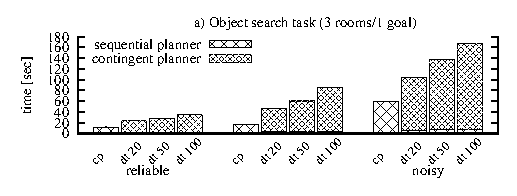
\includegraphics{dora2-time}\hfill
  % \vspace{2mm}
  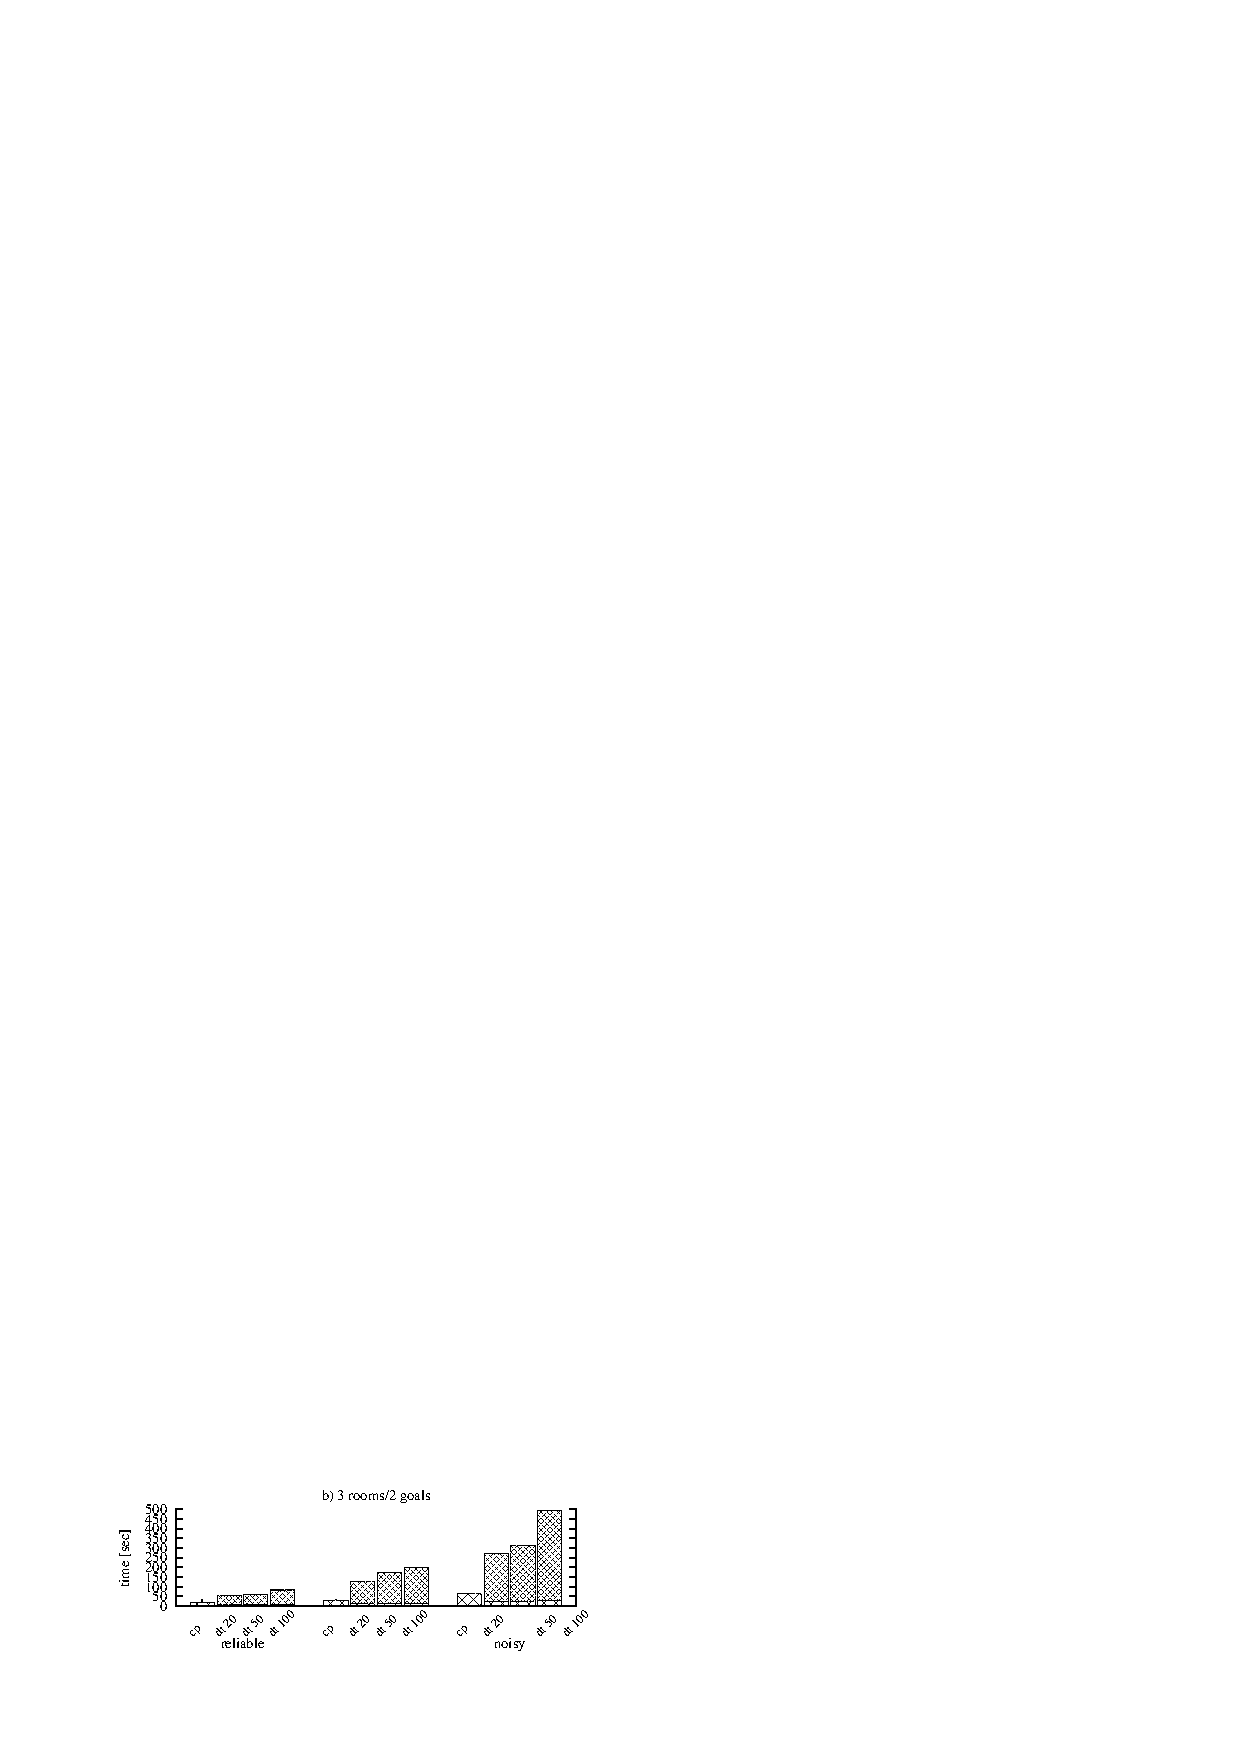
\includegraphics{dora3-time}\hfill
  % \vspace{2mm}
  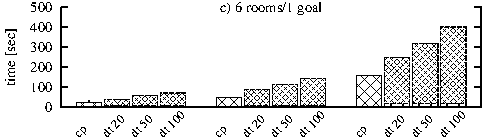
\includegraphics{dora4-time}\hfill
  \vspace{2mm}
  
\includegraphics{dora56-time}\hfill
  % \vspace{2mm}
  % 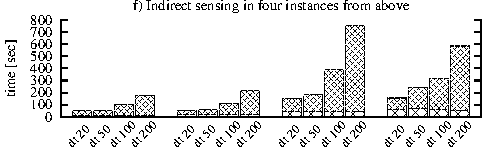
\includegraphics{dora-cat-time}\hfill
  \caption{Average runtime}
  \label{fig:results-time}
\end{figure}

\begin{figure}[h!]
  % \centering
  % 
\includegraphics{dora1-quality}\hfill
  % \vspace{2mm}
  % 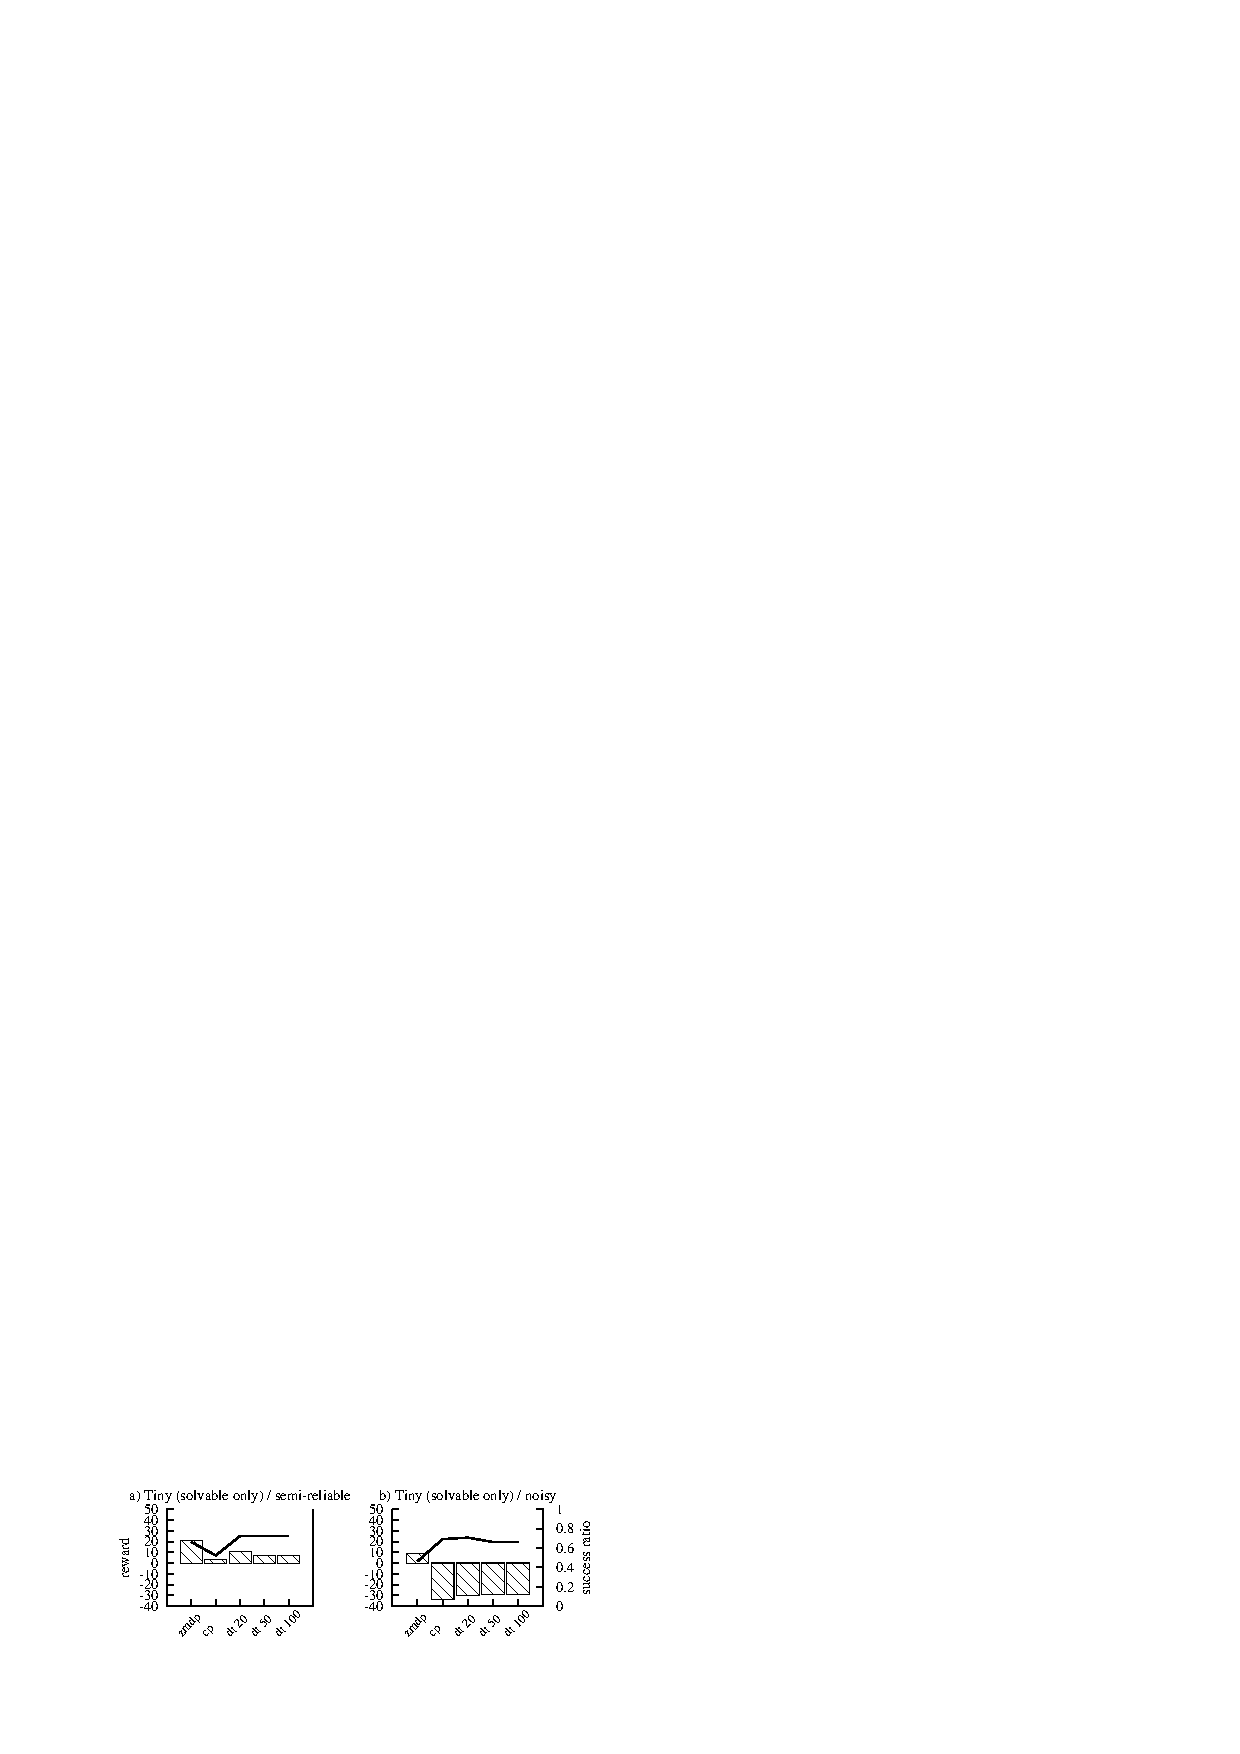
\includegraphics{pomdp-solvable-quality}\hfill
  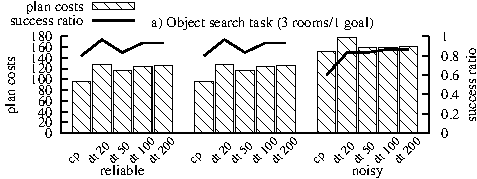
\includegraphics{dora2-quality}\hfill
  % \vspace{2mm}
  
\includegraphics{dora3-quality}\hfill
  % \vspace{2mm}
  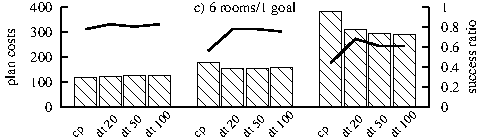
\includegraphics{dora4-quality}\hfill
  \vspace{2mm}
  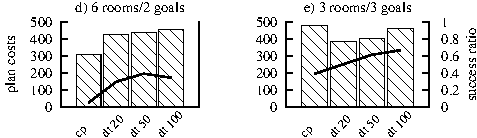
\includegraphics{dora56-quality}\hfill
  \vspace{2mm}
  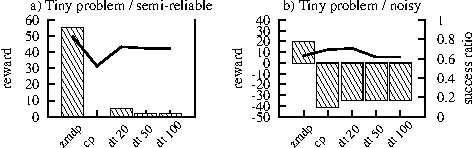
\includegraphics{pomdp-quality}\hfill
  % \vspace{2mm}
  % 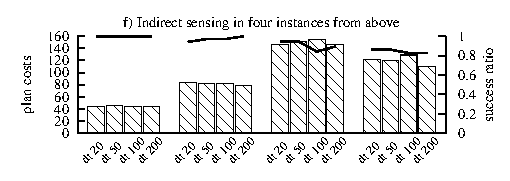
\includegraphics{dora-cat-quality}\hfill
  \caption{Average plan costs and number of successful runs.}
  \label{fig:results-quality}
\end{figure}

We find that if sensing is reliable there is little to be gained
through DT sessions, as the greedy approach of the {\em baseline} is
sufficient. As sensing degrades contingent planning pays off.  Time
spent in DT planning increases steeply as the abstraction $\bstate_0$
becomes more refined.  That refinement seems to be paying off in terms
of the success rate, particularly for tasks $d$ and $e$. For less
refined initial configurations, the increased cost of DT
planning is partially compensated for by a decrease in Fast Downward planning
times. The relatively high success rate irrespective of the level of
refinement in the initial configuration indicates the effectiveness of
using conditional entropy to guide abstraction refinement in our
setting.

%%% Local Variables: 
%%% mode: latex
%%% TeX-master: "aaai11"
%%% End: 


%% \section{Discussion}
%% 

A theoretical criticism of switching continual planning, concerns
interleaved sequential and decision-theoretic sessions failing to make
any progress towards the objective.



\section{Concluding Remarks}


From an automated planning perspective, the problem of practical
mobile robot control poses important and contrary challenges.
%%
On the one hand, planning and execution monitoring must be
lightweight, robust, timely, and should span the lifetime of the
robot. Those processes must seamlessly accommodate exogenous events,
changing objectives, and the underlying unpredictability of the
environment.
%%
On the other hand, robot planning should perform computationally
expensive reasoning about contingencies, and possible revisions of
subjective belief according to quantitatively modelled uncertainty in
acting and sensing. 

In this paper we address these challenges, developing a continual
planner that switches between sequential and decision-theoretic
planning. Given a POMDP model of the environment, sequential planning
is used to compute an initial deterministic sequential plan and
complementary runtime evolution of the decision process. That plan is
executed until a validation of an assumption about a runtime
proposition is requested.


The sequential mode of our system always schedules decision-theoretic
planning before executing actions that are not applicable with
certainty. This is vastly inefficient if the utility of that plan is
not dependent on the actions successful execution. This is the case
where a plan is conformant. Therefore, in the future we must develop a
cheap (heuristic) procedure to evaluate the utility of sensing at
steps in sequential plan.






The switching continual planning system we have described serves as
the underlying planner for CogX.




the effects of a {\em sense} schema are perceptual, whereas the
effects of an {\em operator} schema are over state propositions.




posted by a motivational component of the underlying robotic
architecture. 

contingent sensory plans that are tailored to current
objectives.

In this paper we present an approach to continual planing that uses
two planning systems. The first 

 to a distinct class of
challenges. We suppose 
%%
The underlying environment is modelled as a POMDP. We use the fast
classical satisficing system FastDownward to find a deterministic
sequential plan and complementary runtime evolution of that
process. This corresponds to a generalisation of replanning in
probabilistic planning to problems with partial observability.

Interaction between the sequential planner and execution proceeds
more-or-less analogously to popular replanning approaches

Addressing these challenges in a monolithic framework, we present a
{\em switching} continual planner, that uses the fast sequential
satisficing procedure FastDownward to perform net-benefit
%%
makes reasonable assumptions about the evolution of the runtime state
given a POMDP model of the environment. 

contingent sensory plans that are tailored to current
objectives.


The decision-theoretic planner is able to tailor sensory processing on
a robot platform to the current objective, while FastDownward  quickly 


In this paper we develop a continual planing system that uses two
planning systems. The first, is a state-of-the-art domain independent
planner for deterministic problems. The second is a information-state
contingency planning the information-state space of 


Continual planning is a powerful technique that goes some way to
addressing those challenges. That approach interleaves planning and
execution, deliberately postponing planning for contingencies unless
they eventuate during execution. 


computing a single sequential plan and
eventuality



To these challenges it seems a continual planning approach is best, 

where the runtime state evolves during plan execution 


interleaved planning and execution. 

the latter is able to tailor sensory processing on a robot platform,
in order that it.

{\em ad-hoc} 

, reason about degrees of belief and uncertainty about the world, 

probabilistic sequential decision making in practical sized problems
is intractable.

quantitative probabilistic models of the perception and action .



\bibliographystyle{aaai}
\bibliography{papers}

\end{document}


























\subsection{PPDDL}

We briefly discuss the description language PPDDL, a fairly
straight-forward extension of the Planning Domain Definition Language
for describing fully observable Markov decision processes.

\small{
\begin{tabtt}
(\= :action look-at-object \\
  \> :parameters \=(?r - robot ?v - visual-object\\
  \> \> ?l - label ?l - location) \\
  \> :precondition (and (= (is-in ?r) ?l) \\
  \> \> (= (label ?o) ?l) ) \\
  \> :effect (and (assign (reward) -3) ) ) \\
\end{tabtt}
}

\small{
\begin{tabtt}
(\= :observe visual-object \\
  \> :parameters \=(?r - robot ?v - visual-object\\
  \> \> ?l - label ?l - location) \\
  \> :execution (look-at-object ?r ?v ?l ?l) \\
  \> :effect (when (= (is-in ?o) ?l) (probabilistic 0.8)) \\
\end{tabtt}
}

\small{
\begin{tabtt}
(\= :sensor look-for-object \\
  \> :agent (?a - robot) \\
  \> :parameters (?l - label ?l - location) \\
  \> :variables (?o - visual-object) \\
  \> :precondition (\=and (= (is-in ?r) ?l) \\
  \> \> (= (label ?o) ?l) (assume (is-in ?o) ?l) ) \\
  \> :effect () \\
  \> :sense (= (is-in ?o) ?l) \\
\end{tabtt}
}

\subsection{MAPL}



%% \scriptsize
%% \begin{nopagebreak}\begin{tabtt}
%% <observation-def> \=::= \=(:sense <observation symbol> \\
%%                         \> \> :parameters (<typed list (variable)>)  \\
%%                         \> \> <o-def body>) \\
%%   <o-symbol> \> ::= <name> \\
%%   <o-def body> \> ::= [:precondition <GD>] \\
%%   \> \> [:execution <atomic action(term)> ] \\
%%     \> \> [:effect <o-effect>] \\
%%   <atomic action(t)> \> ::= (<action symbol> t\zom) \\
%%   <o-effect> \> ::= (and <c-o-effect>\zom) \\
%%   <o-effect> \> ::= <c-o-effect> \\
%%   <c-o-effect> \> ::= \req{:probabilistic-effects} (probabilistic <prob> <o-effect>) \\
%%   <c-o-effect> \> ::= <p-o-effect> \\
%%   <atomic o-formula(t)> \> ::= (<observation> t\zom) \\
%%   <p-o-effect> \> ::= <atomic o-formula(term)> \\
%%   <p-o-effect> \> ::= (not <atomic o-formula(term)>) \\
%%   <o-f-comp> \> ::= (<binary-comp> <o-f-exp> <o-f-exp>)\\
%%   <o-f-exp> \> ::= <number>\\
%%   <o-f-exp> \> ::= (- <o-f-exp>)\\
%%   <o-f-exp> \> ::= <o-f-head>\\
%%   <o-f-head> \> ::= (<o-function-symbol> <term>\zom )\\
%%   <o-f-head> \> ::= <o-function-symbol>\\
%% \end{tabtt}\end{nopagebreak}
%% \noteme{<structure-def> ::= <attach-def>}
%% \normalsize



%% \footnote{We have simplified the schemata for illustrative
%% purposes. In practice, the probabilities of a particular observation
%% here should be parametrised by the type of visual object the robot is
%% searching for, and category of the location.}


We suppose $\bstate_0$ is given in a factored tree format of the
form:


%% \small{
%% \begin{tabtt}
%% (:init  (and \=f_{11} f_{12} ..
%%  \> (probabilistic p_{}) 
%%  \> (probabilistic ..) ..) \\
%% \end{tabtt}
%% }

%% \[(:\pp{init} (and f_{11} f_{12} .. (\pp{probabilistic} p_) ))\]


planning in practical sized POMDPs is intractable. One approach is to
described the task hierarchically, thereby constrain and simplify the
policy search task. The approach ~\cite{}. 


%% More generally, a useful
%% formalism for representing solutions to POMDPs is the finite-state
%% controller (FSC). This is a three-tuple $\langle \nodes, \selection,
%% \transition \rangle$ where: $\node \in \nodes$ is a set of nodes,
%% $\selection_\node(\action) = P(\action | \node)$, and
%% $\transition_\node(\action, \observation, \node') = P(\node'|\node,
%% \action, \observation)$. Where the value of acting is the discounted
%% accumulated reward over an infinite horizon, then each controller can
%% be assigned a value, written $V_\node(\state)$, expressed in the usual
%% way according to the Bellman equation:

%% \begin{equation}\label{eq:evaluation}
%% \begin{array}{lcl}
%% V_\node(\state) & = & \sum_{\action \in \actions}
%% \selection_\node(\action) \reward(\state, \action) \;\; + \vspace{1ex} \\

%% && \hspace{-10ex} \beta \sum_{\action, \observation,
%% \state', \node'} \transition_\node(\action, \observation, \node')
%% \transProb(\state, \action, \state') \obsDist_\observ(\state',
%% \action) V_{\node'}(\state')
%% \end{array}
%% \end{equation}

%% \noindent Here, the value of {\em prior} $\bstate$ given an FSC is
%% then:

%% \begin{equation} \label{eq:valueBelief}
%% V_{\pp{FSC}}(\bstate) = \max_{\node \in \nodes} \sum_{\state \in \states} \bstate(\state) V_\node(\state)
%% \end{equation}

%% \noindent There is a corresponding deterministic FSCs for both
%% sequential (i.e., conformant) and contingent
%% plans. Eq~\ref{eq:evaluation} gives their value in the finite-horizon
%% case, if we take $\beta = 1$, and alter the process dynamics so there
%% is a compulsory transition to a zero utility sink state when that
%% horizon is reached.


 ---i.e., the values of {\em
runtime variables} in the continual paradigm--- are treated , and
therefore plan for a specific eventuality, replanning from scratch if
something




Sequential planning in our approach proceeds in two phases. In the
first phase, the goal is to identify a plan prefix

In sequential planning, the plan prefix corresponds to choosing a
valid abstract starting state. 

moreover, for the purpose of decision-theoretic abstractions, 


A relaxed form of {\em visitation} we call {\em abstract
  visitation}. In the abstract case a conjunctive term is visited
  provided all its atomic subterms are visited, and zero or more of
  its probabilistic terms are visited.

The planner has a compulsory starting action, that visits the root
term, and then has to execute visitation actions until that plan
prefix corresponds to a valid {\em abstract visitation} of the {\em
:init} decleration. Beyond such a prefix, the process actions and senses are
available to the planner 


Goal expressions in the problem description ---for example
$(\pp{kval}~(\pp{location}~\pp{box}))$ expresses ``the robot knows the
location of the {\em box}--- are treated as control-knowledge by the
planner. Here, a plan is not considered valid unless in the finial
stet the goal condition is satisfied.
